\section{Experimental setup}
Like mentioned at the beginning the main goal of this experiment is to measure the absorption spectrum of rubidium.
In the following we will present the experimental setup that allows at the end to measure the intensity of a laser beam
behind a gas cell as a function of frequency. The single steps of calibration and experimental results will be discussed
in the next section. 

The optical grating of the extrenal cavity has two knobs for vertical and horizontal alignment. The vertical alignment 
is important to make sure that the laser beam is in the same plane like the thin active zone of the diode. To optimize the adjustment 
we use a CCD camera which enables us to differ between normal LED emission and lasing. The adjustment is perfect, when the 
threshold $I_{th}$ reaches a minimum. 

The length $L$ of the external cavity can be varied with a piezo modulator. The expansion of piezo crystals can be manipulated by an
applied voltage. Using a triangular voltage signal we can execute a periodic variation of $L$ and thus a sweep in laser frequeny. The
modulation can be applied to the piezo or simultaniously to the diode current.

The overall setup is displayed in figure~\ref{fig: setup}. To get gasious 
rubidium, the cell is heated. With the CCD camera placed infront of the cell it is possible to find the 
right adjustment that leads to a lasing wavelength that is absorbed. Photoluminescence becomes visible in this case.  
The laser intensity is measured with photodiodes since the photo current
is propotional to the incoming light intensity. The signals are displayed with a digital oscilloscope. 
Although one photodiode would be sufficient to observe the effect of the gas absorption we use in the end 
a second diode (see figure~\ref{fig: setup}). A beam splitter before the gas cell directs \SI{50}{\percent}
of the laser intensity in the second photo diode without passing the gas cell. This procedure is motivated by the 
condition that the piezo modulation is also connected with a modulation of the overall laser intensity. Subtracting 
the signal of photo diode one and two produces a new signal that is showing us the clean influence of the gas.

\begin{figure}
\centering
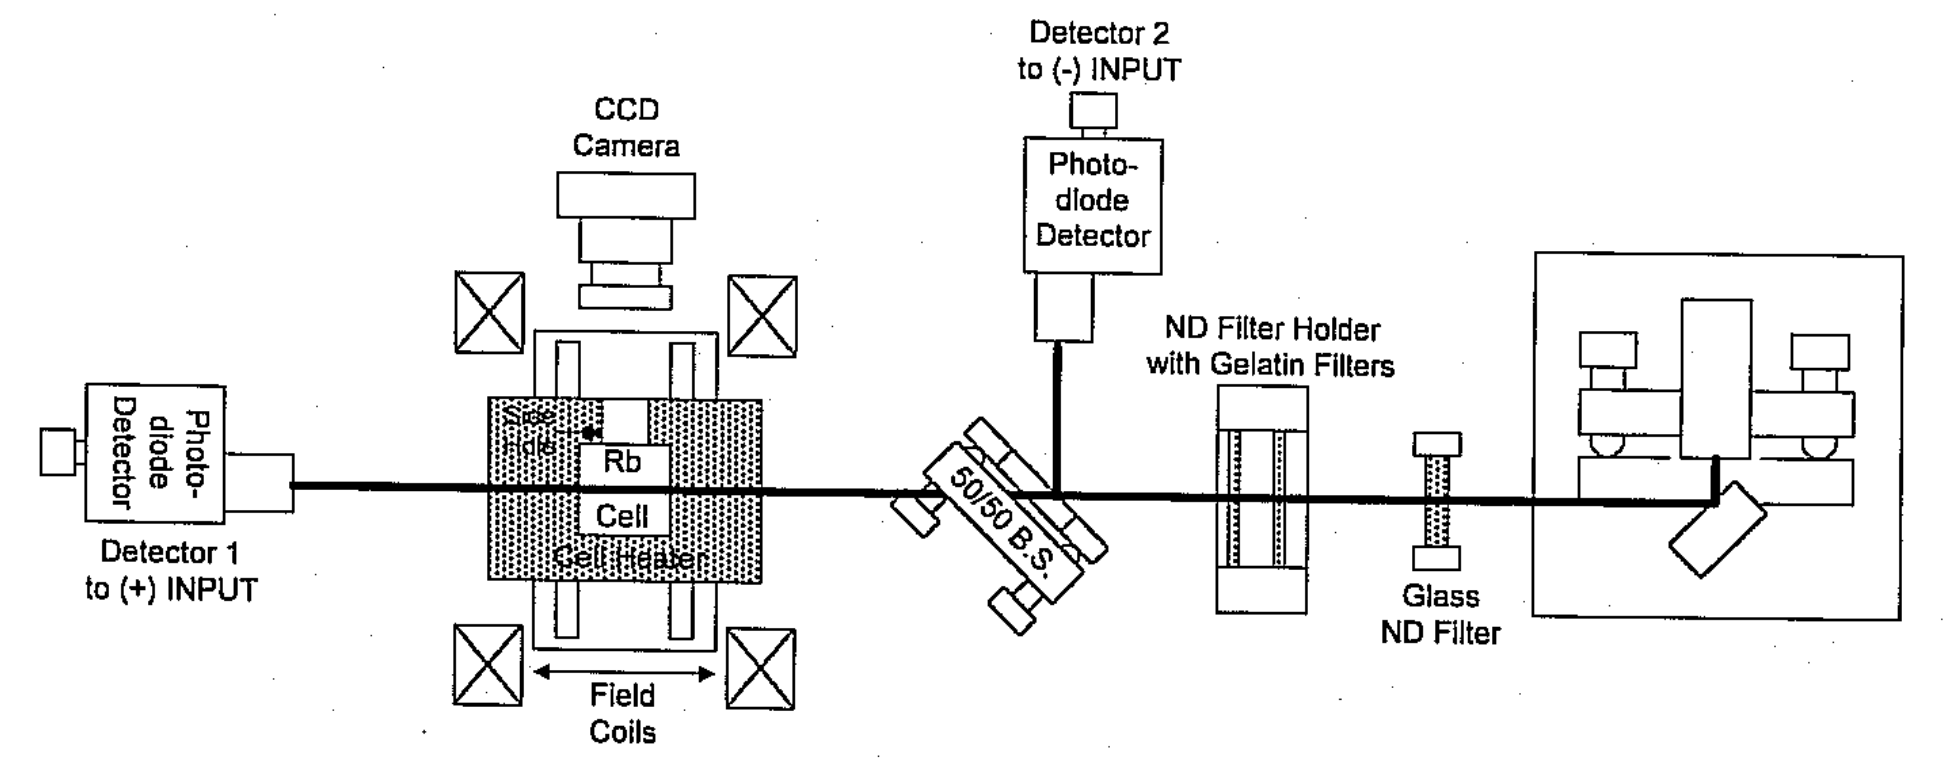
\includegraphics[width = \textwidth]{pics/setup.png}
\caption{Experimental setup for measuring the absorption spectrum of gaseous rubidium. Threw the calibration 
process not all components are used in each step (see section~\ref{} for details) \cite{anleitung60}. }
\label{fig: setup}
\end{figure}



